\documentclass[10pt]{beamer}
\usetheme{Madrid}
\usecolortheme{default}
\usepackage{subcaption}
\usepackage{caption}
\captionsetup{font=small, labelfont=bf}
\captionsetup[sub]{labelsep=period, subrefformat=brace}
\usepackage{graphicx}
\usepackage{amsmath,amssymb}
\usepackage{bm}
\usepackage{tikz}

\usetikzlibrary{shapes,arrows,positioning,calc}
\tikzset{
    block/.style = {draw, rectangle, minimum height=1.2cm, minimum width=2cm, align=center},
    sum/.style = {draw, circle, node distance=1cm},
    input/.style = {coordinate},
    output/.style = {coordinate},
    spring/.style = {decorate, decoration={coil, amplitude=3pt, segment length=3pt}},
}
\usepackage{booktabs}

% Title page info
\title{Robot Motion and Force Control}
\subtitle{From Independent Joints to Operational Space and Interaction Control}
\author{Your Name}
\institute{Your Institution}
\date{\today}

% Define commands for robot dynamics
\newcommand{\vect}[1]{\boldsymbol{#1}}
\newcommand{\M}{\vect{M}}
\newcommand{\C}{\vect{C}}
\newcommand{\g}{\vect{g}}
\newcommand{\q}{\vect{q}}
\newcommand{\qd}{\vect{q}_d}
\newcommand{\qdot}{\dot{\vect{q}}}
\newcommand{\qddot}{\ddot{\vect{q}}}
\newcommand{\tauvec}{\vect{\tau}}
\newcommand{\x}{\vect{x}}
\newcommand{\xd}{\vect{x}_d}
\newcommand{\J}{\vect{J}}
\newcommand{\F}{\vect{F}}
\newcommand{\Kp}{\vect{K}_p}
\newcommand{\Kd}{\vect{K}_d}
\newcommand{\Ki}{\vect{K}_i}

\begin{document}



\section{Actuators in Robotics}
\begin{frame}{Actuators: The "Muscles" of Robots}
    \begin{block}{Definition}
        Actuators convert energy into mechanical motion. They provide the \textbf{force/torque} to move robot joints.
    \end{block}
    
    \begin{columns}
        \begin{column}{0.5\textwidth}
            \begin{exampleblock}{Main Types}
                \begin{enumerate}
                    \item \textbf{Electric Motors}
                    \begin{itemize}
                        \footnotesize
                        \item DC Motors (Brushed/Brushless)
                        \item Stepper Motors
                        \item Servo Motors
                    \end{itemize}
                    \item \textbf{Hydraulic Actuators}
                    \item \textbf{Pneumatic Actuators}
                    \item \textbf{Smart Material Actuators}
                    \begin{itemize}
                        \footnotesize
                        \item Piezoelectric
                        \item Shape Memory Alloys
                    \end{itemize}
                \end{enumerate}
            \end{exampleblock}
        \end{column}
        
        \begin{column}{0.5\textwidth}
            \begin{figure}
            % DC Motor
            \centering
                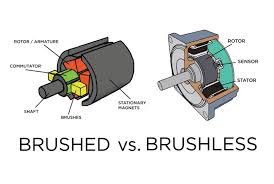
\includegraphics[width=0.5\textwidth]{./robotique_figures/brushed_brushless_actuator}           
            \end{figure}
            \begin{figure}
            \centering
                    % Stepper
                    \begin{subfigure}[b]{0.16\textwidth}
                     \centering
                    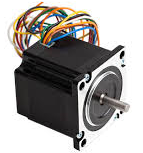
\includegraphics[scale=0.4]{./robotique_figures/stepper_motor.png}
                    \end{subfigure}
                \quad
                    \begin{subfigure}[b]{0.16\textwidth}
                    \centering
                    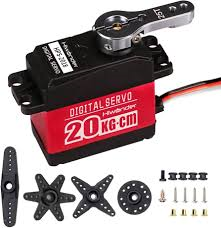
\includegraphics[scale=0.4]{./robotique_figures/servo_motors.png} 
                    \end{subfigure}           
            \end{figure}
        \end{column}
    \end{columns}
\end{frame}

\begin{frame}{Electric Motors: The Most Common Choice}
\small               % Reduce overall text size
\setlength{\tabcolsep}{4pt} % Reduce column spacing
\renewcommand{\arraystretch}{0.9} % Reduce row height

\begin{table}
\centering
\begin{tabular}{p{0.28\textwidth} p{0.32\textwidth} p{0.32\textwidth}}
\toprule
\textbf{Type} & \textbf{Advantages} & \textbf{Disadvantages} \\
\midrule

\textbf{DC Brushed} &
\begin{itemize}\footnotesize
    \item Simple control
    \item Low cost
    \item High torque at low speed
\end{itemize} &
\begin{itemize}\footnotesize
    \item Brush wear
    \item EMI
    \item Maintenance
\end{itemize} \\

\textbf{DC Brushless} &
\begin{itemize}\footnotesize
    \item High efficiency
    \item Long life
    \item High power density
\end{itemize} &
\begin{itemize}\footnotesize
    \item Complex control
    \item Higher cost
    \item Needs encoder
\end{itemize} \\

\textbf{Stepper} &
\begin{itemize}\footnotesize
    \item Open-loop control
    \item Good position accuracy
    \item High holding torque
\end{itemize} &
\begin{itemize}\footnotesize
    \item Resonance issues
    \item Low efficiency
    \item Can lose steps
\end{itemize} \\
\bottomrule
\end{tabular}
\end{table}

\vspace{-2mm}

\textbf{Key Parameters}
\footnotesize
\begin{itemize}
    \item \textbf{Torque Constant} ($K_t$): Nm/A
    \item \textbf{Back-EMF Constant} ($K_e$): V/(rad/s)
    \item \textbf{Rated Torque/Speed}
    \item \textbf{Power Density}: W/kg
\end{itemize}
\end{frame}


\begin{frame}{Hydraulic vs. Pneumatic Actuators}
    \begin{columns}
        \begin{column}{0.48\textwidth}
            \begin{block}{Hydraulic Actuators}
                \begin{center}
                    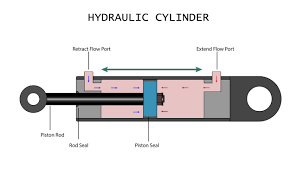
\includegraphics[scale=0.5]{./robotique_figures/hydraulic_cylinder.png}
                \end{center}
                \begin{itemize}
                    \item \textbf{Very high force/torque}
                    \item Good stiffness
                    \item Can be leaky, messy
                    \item Needs pump, reservoir
                    \item \textbf{Applications:} Excavators, heavy lifting
                \end{itemize}
            \end{block}
        \end{column}
        
        \begin{column}{0.48\textwidth}
            \begin{block}{Pneumatic Actuators}
                \begin{center}
                     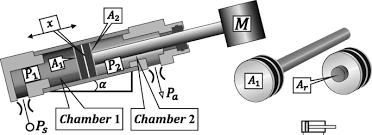
\includegraphics[scale=0.4]{./robotique_figures/pneumatic cylinder.png}
                \end{center}
                \begin{itemize}
                    \item \textbf{Fast, clean}
                    \item Lower force than hydraulic
                    \item Compressible $\Rightarrow$ less stiff
                    \item Needs compressor, dryer
                    \item \textbf{Applications:} Pick-and-place, assembly
                \end{itemize}
            \end{block}
        \end{column}
    \end{columns}
    
    \vspace{5mm}
    \begin{alertblock}{Modern Trend: Electro-Hydrostatic Actuators (EHA)}
        Electric motor + pump + cylinder in one package. Best of both worlds!
    \end{alertblock}
\end{frame}

\section{Sensors for Motion Sensing}
\begin{frame}{Sensors of Robots}
    \begin{block}{Motion Sensing}
        \begin{itemize}
            \item \textbf{Joint-level sensing:} Where is each joint?
            \item \textbf{End-effector sensing:} Where is the tool?
            \item \textbf{Environment sensing:} What's around the robot?
        \end{itemize}
    \end{block}
    
    \begin{columns}
        \begin{column}{0.5\textwidth}
            \begin{exampleblock}{Position/Velocity Sensors}
                \begin{itemize}
                    \item \textbf{Encoders}
                    \begin{itemize}
                        \footnotesize
                        \item Incremental
                        \item Absolute
                    \end{itemize}
                    \item \textbf{Potentiometers}
                    \item \textbf{Resolvers}
                    \item \textbf{LVDT/RVDT}
                    \item \textbf{Hall Effect Sensors}
                \end{itemize}
            \end{exampleblock}
        \end{column}
        
        \begin{column}{0.5\textwidth}
            \begin{exampleblock}{Force/Torque Sensors}
                \begin{itemize}
                    \item \textbf{Strain Gauges}
                    \item \textbf{Load Cells}
                    \item \textbf{Force-Torque Sensors}
                    \item \textbf{Tactile Sensors}
                    \item \textbf{Pressure Sensors}
                \end{itemize}
            \end{exampleblock}
        \end{column}
    \end{columns}
\end{frame}

\begin{frame}{Encoders: joint position sensors}
    \begin{columns}
        \begin{column}{0.5\textwidth}
            \begin{block}{Incremental Encoders}
                \begin{center}
                    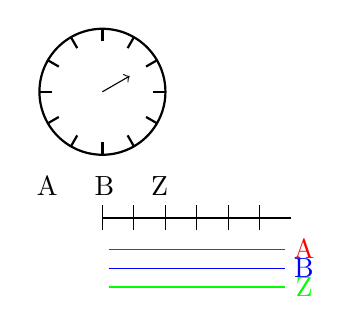
\begin{tikzpicture}[scale=0.8]
                        \draw[thick] (0,0) circle (1);
                        \foreach \i in {0,30,...,330} {
                            \draw[thick] (\i:0.8) -- (\i:1);
                        }
                        \draw[->] (0,0) -- (30:0.5);
                        \node at (0,-1.5) {A \quad B \quad Z};
                        \draw[thick] (0,-2) -- (3,-2);
                        \foreach \i in {0,0.5,1,1.5,2,2.5} {
                            \draw (\i,-1.8) -- (\i,-2.2);
                        }
                        \draw[red] (0.1,-2.5) -- (2.9,-2.5);
                        \draw[blue] (0.1,-2.8) -- (2.9,-2.8);
                        \draw[green] (0.1,-3.1) -- (2.9,-3.1);
                        \node[red] at (3.2,-2.5) {A};
                        \node[blue] at (3.2,-2.8) {B};
                        \node[green] at (3.2,-3.1) {Z};
                    \end{tikzpicture}
                \end{center}
                \begin{itemize}
                    \footnotesize
                    \item Pulses per revolution (PPR)
                    \item Channels A, B (quadrature)
                    \item Index channel Z
                    \item Need homing
                \end{itemize}
            \end{block}
        \end{column}
        
        \begin{column}{0.5\textwidth}
            \begin{block}{Absolute Encoders}
                \begin{center}
                    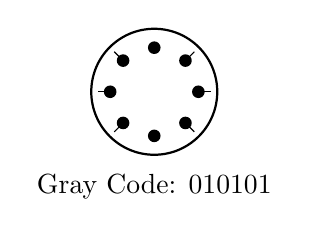
\begin{tikzpicture}[scale=0.8]
                        \draw[thick] (0,0) circle (1);
                        \foreach \i in {0,45,...,315} {
                            \fill (\i:0.7) circle (0.1);
                        }
                        \draw (0:0.7) -- (0:0.9);
                        \draw (45:0.7) -- (45:0.9);
                        \draw (135:0.7) -- (135:0.9);
                        \draw (180:0.7) -- (180:0.9);
                        \draw (225:0.7) -- (225:0.9);
                        \draw (315:0.7) -- (315:0.9);
                        \node at (0,-1.5) {Gray Code: 010101};
                    \end{tikzpicture}
                \end{center}
                \begin{itemize}
                    \footnotesize
                    \item Unique code per position
                    \item No homing needed
                    \item Single-turn vs multi-turn
                    \item More expensive
                \end{itemize}
            \end{block}
        \end{column}
    \end{columns}
    
    \begin{alertblock}{Encoder Resolution}
        $\Delta\theta = \frac{360^\circ}{\text{PPR} \times 4}$ (with quadrature decoding)
    \end{alertblock}
\end{frame}

\begin{frame}{Force/Torque and Vision Sensors}
\small

\begin{columns}
    \begin{column}{0.49\textwidth}
        \begin{block}{Force-Torque Sensors}
            \begin{center}
                 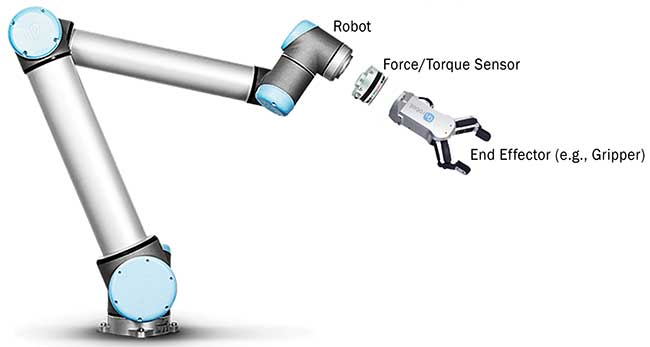
\includegraphics[width=0.65\linewidth]{./robotique_figures/force_torque_sensor.jpg}
            \end{center}
            \vspace{-2mm}
            \begin{itemize}\footnotesize
                \item Measures $F_x, F_y, F_z, M_x, M_y, M_z$
                \item Strain gauge based
                \item Mounted at wrist
                \item Critical for force control
            \end{itemize}
        \end{block}

        \begin{block}{Other Sensors}
            \vspace{-2mm}
            \begin{itemize}\footnotesize
                \item \textbf{Proximity:} Inductive, capacitive
                \item \textbf{LIDAR:} For mapping, navigation
                \item \textbf{IMU:} Accelerometer, gyro
                \item \textbf{Torque Sensors:} In joint
            \end{itemize}
        \end{block}
    \end{column}
    
    \begin{column}{0.49\textwidth}
        \begin{block}{Vision Systems}
            \begin{center}
                 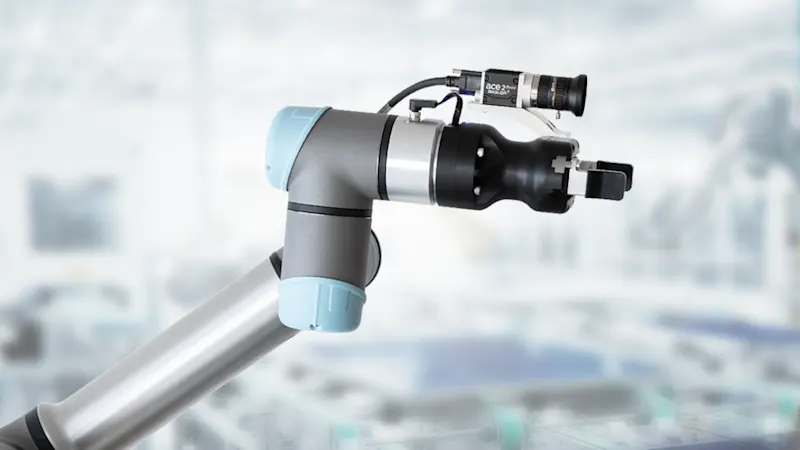
\includegraphics[width=0.65\linewidth]{./robotique_figures/camera_vision_sensors.png}
            \end{center}
            \vspace{-2mm}
            \begin{itemize}\footnotesize
                \item 2D/3D vision
                \item Eye-in-hand vs fixed
                \item For guidance, inspection
                \item Often with LED lighting
            \end{itemize}
        \end{block}
    \end{column}
\end{columns}
\end{frame}


\section{Motion Transmission Mechanisms}
\begin{frame}{Why Transmission Mechanisms?}
    \begin{block}{The Motor-Robot Interface Problem}
        \begin{itemize}
            \item Motors have \textbf{high speed, low torque}
            \item Robots need \textbf{low speed, high torque}
            \item Need \textbf{gear reduction} (typically 50:1 to 200:1)
            \item Also need to \textbf{transmit motion} to different locations
        \end{itemize}
    \end{block}
    
    \begin{columns}
        \begin{column}{0.5\textwidth}
            \begin{exampleblock}{Common Mechanisms}
                \begin{enumerate}
                    \item Gears (Spur, Planetary, Harmonic)
                    \item Belts and Pulleys
                    \item Chains and Sprockets
                    \item Lead/Ball Screws
                    \item Cable Drives
                    \item Linkages
                \end{enumerate}
            \end{exampleblock}
        \end{column}
        
        \begin{column}{0.5\textwidth}
            \begin{alertblock}{Key Metrics}
                \begin{itemize}
                    \footnotesize
                    \item \textbf{Gear Ratio} ($N$)
                    \item \textbf{Efficiency} ($\eta$)
                    \item \textbf{Backlash}
                    \item \textbf{Stiffness}
                    \item \textbf{Mass/Inertia}
                \end{itemize}
            \end{alertblock}
        \end{column}
    \end{columns}
\end{frame}

\begin{frame}{Gear Mechanisms}
    \begin{columns}
        \begin{column}{0.33\textwidth}
            \begin{block}{Spur Gears}
                \begin{center}
                    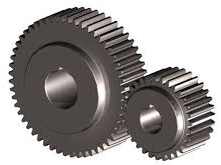
\includegraphics[scale=0.3]{./robotique_figures/spur_gears.png}
                \end{center}
                \begin{itemize}
                    \footnotesize
                    \item Parallel shafts
                    \item $N = N_2/N_1$
                    \item Simple, efficient
                    \item Can have backlash
                \end{itemize}
            \end{block}
        \end{column}
        
        \begin{column}{0.33\textwidth}
            \begin{block}{Planetary Gears}
                \begin{center}
                 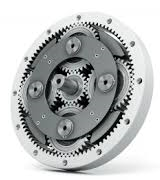
\includegraphics[scale=0.3]{./robotique_figures/planetary_gears.png}   
                \end{center}
                \begin{itemize}
                    \footnotesize
                    \item High reduction in small package
                    \item Multiple power paths
                    \item High torque density
                    \item Complex, expensive
                \end{itemize}
            \end{block}
        \end{column}
        
        \begin{column}{0.33\textwidth}
            \begin{block}{Harmonic Drive}
                \begin{center}
                    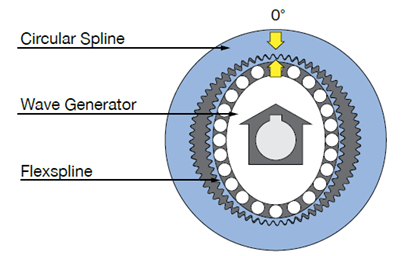
\includegraphics[scale=0.2]{./robotique_figures/harmonic_drive.png} 
                \end{center}
                \begin{itemize}
                    \footnotesize
                    \item \textbf{Zero backlash}
                    \item Very high ratios (50:1 to 320:1)
                    \item High precision
                    \item Limited torque, expensive
                    \item Used in robot wrist joints
                \end{itemize}
            \end{block}
        \end{column}
    \end{columns}
    
    \vspace{3mm}
    \begin{alertblock}{Gear Ratio Effects}
        \begin{itemize}
            \item \textbf{Torque:} $\tau_{out} = N*\eta*\tau_{in}$
            \item \textbf{Speed:} $\omega_{out} = \omega_{in}/N$
            \item \textbf{Reflected Inertia:} $J_{reflected} = J_{motor} \times N^2$
        \end{itemize}
    \end{alertblock}
\end{frame}

\begin{frame}{Belts, Pulleys, and Other Transmissions}
\small

\begin{columns}[t]

    % LEFT COLUMN ---------------------------------------------------
    \begin{column}{0.48\textwidth}

        % --- SAME POSITION, OVERLAY SWITCHING ---
        \only<1>{
        \begin{block}{Timing Belts \& Pulleys}
            \centering
            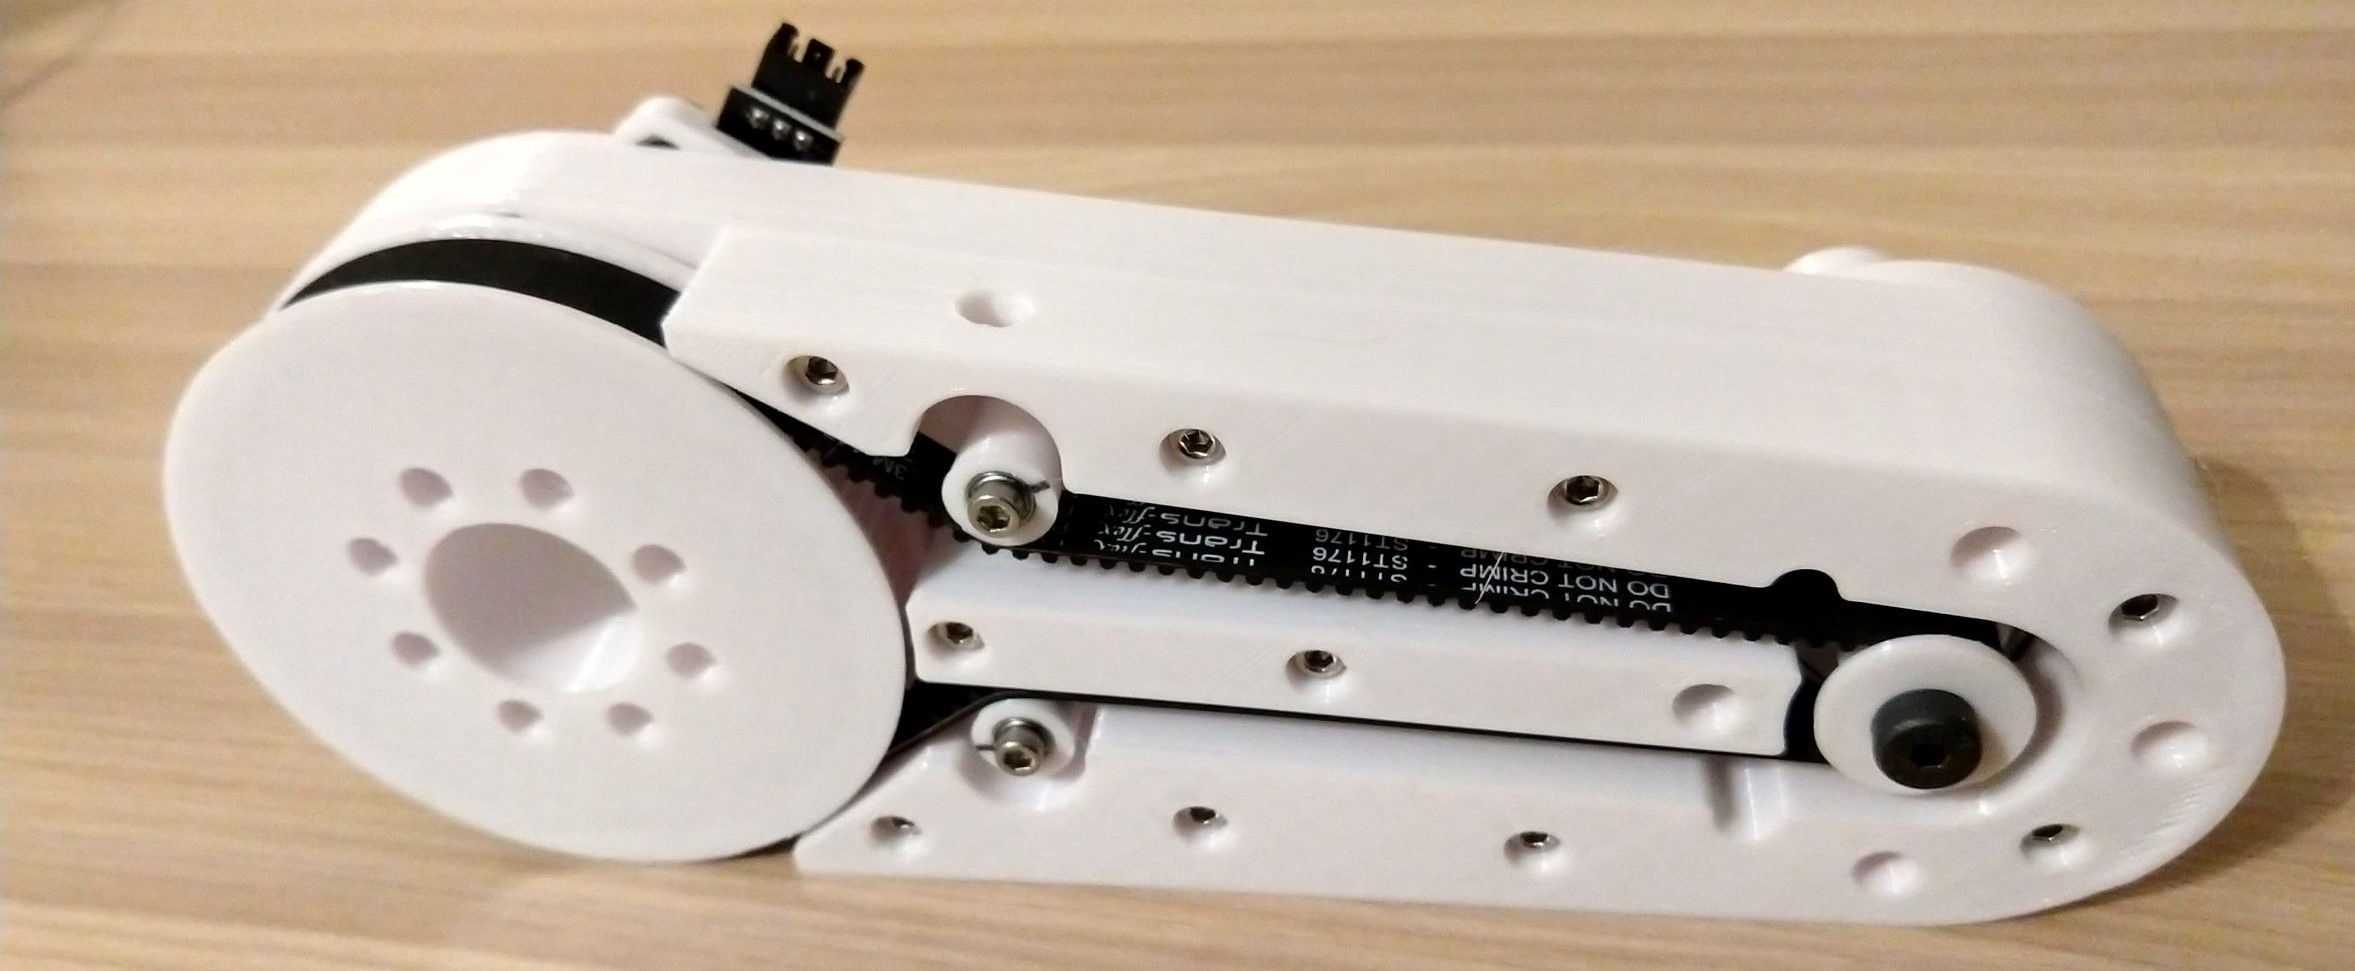
\includegraphics[width=0.55\linewidth]{./robotique_figures/pulley_belt_transmission.jpg}
            \vspace{-2mm}
            \begin{itemize}\footnotesize
                \item \textbf{Synchronous} (no slip)
                \item Good for long distances
                \item Low backlash
                \item Needs tensioning
            \end{itemize}
        \end{block}
        }

        \only<2>{
        \begin{block}{Ball Screws}
            \centering
            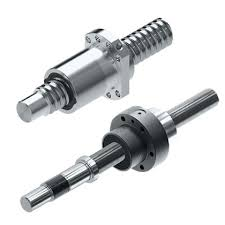
\includegraphics[width=0.60\linewidth]{./robotique_figures/ball_screw.jpg}
            \vspace{-2mm}
            \begin{itemize}\footnotesize
                \item Converts rotation to translation
                \item High efficiency (90\%+)
                \item Zero backlash possible
                \item Used in linear axes
            \end{itemize}
        \end{block}
        }

    \end{column}

    % RIGHT COLUMN ---------------------------------------------------
    \begin{column}{0.48\textwidth}

        % --- SAME POSITION, OVERLAY SWITCHING ---
        \only<1>{
        \begin{block}{Cable Drives}
            \centering
            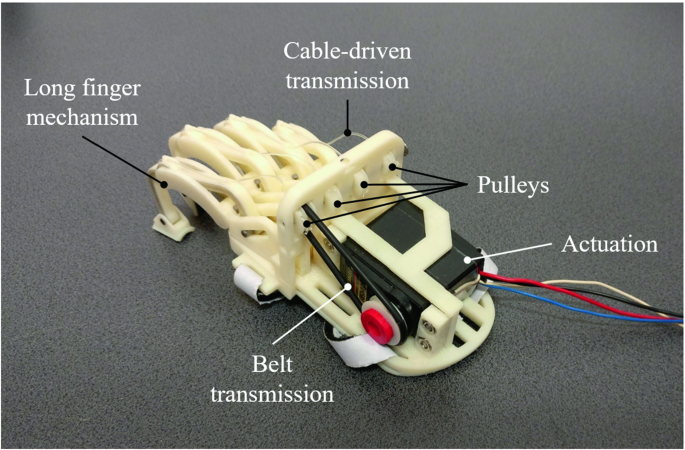
\includegraphics[width=0.60\linewidth]{./robotique_figures/cable_driven_transmission.png}
            \vspace{-2mm}
            \begin{itemize}\footnotesize
                \item \textbf{Remote actuation}
                \item Low inertia at moving part
                \item Used in surgical robots
                \item Needs tensioning, can stretch
            \end{itemize}
        \end{block}
        }

        \only<2>{
        \begin{block}{Direct Drive}
            \centering
            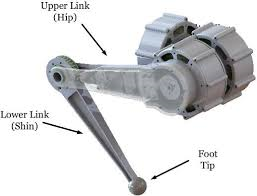
\includegraphics[width=0.55\linewidth]{./robotique_figures/direct_drive.png}
            \vspace{-2mm}
            \begin{itemize}\footnotesize
                \item \textbf{No gears} – motor directly connected
                \item Zero backlash, high stiffness
                \item Needs high-torque motor
                \item Used in precision applications
            \end{itemize}
        \end{block}
        }

    \end{column}
\end{columns}

\end{frame}






\section{End Effectors for Industrial Robots}
\begin{frame}{End Effectors: The "Hands" of Robots}
    \begin{block}{Definition}
        End effectors are devices mounted at the robot wrist that \textbf{interact with the environment} to perform tasks.
    \end{block}
    
    \begin{columns}
        \begin{column}{0.5\textwidth}
            \begin{exampleblock}{Two Main Categories}
                \begin{enumerate}
                    \item \textbf{Grippers}
                    \begin{itemize}
                        \footnotesize
                        \item Mechanical
                        \item Vacuum
                        \item Magnetic
                        \item Adhesive
                    \end{itemize}
                    \item \textbf{Tools}
                    \begin{itemize}
                        \footnotesize
                        \item Welding
                        \item Painting
                        \item Drilling
                        \item Dispensing
                    \end{itemize}
                \end{enumerate}
            \end{exampleblock}
        \end{column}
        
        \begin{column}{0.5\textwidth}
           \begin{center}
               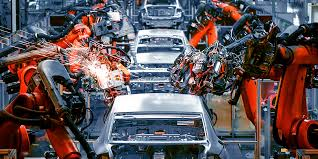
\includegraphics[scale=0.43]{./robotique_figures/robots_grippers1.png}
               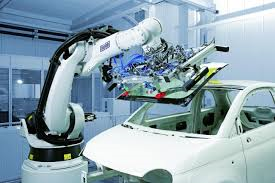
\includegraphics[scale=0.43]{./robotique_figures/robot_grippers2.png}
           \end{center}
        \end{column}
    \end{columns}
    
    \begin{alertblock}{Tool Changers}
        Allow one robot to use multiple end effectors automatically. Critical for flexible automation.
    \end{alertblock}
\end{frame}

\begin{frame}{Mechanical Grippers: The Most Common Type}

\begin{columns}[t]
    \begin{column}{0.48\textwidth}
        \begin{block}{Two-Finger Grippers}
            \begin{center}
                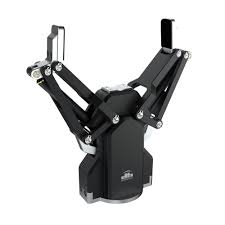
\includegraphics[width=0.2\linewidth]{robotique_figures/two_finger.png}
            \end{center}
            \footnotesize
            \begin{itemize}
                \item Parallel or angular jaws
                \item Self-centering options
                \item Pneumatic, electric, or hydraulic actuation
            \end{itemize}
        \end{block}
    \end{column}

    \begin{column}{0.48\textwidth}
        \begin{block}{Three-Finger Grippers}
            \begin{center}
                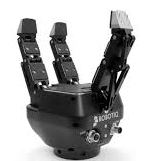
\includegraphics[width=0.2\linewidth]{robotique_figures/three_fingers.png}
            \end{center}
            \footnotesize
            \begin{itemize}
                \item Better centering accuracy
                \item Increased contact points
                \item Suitable for irregular shapes
                \item Mechanically more complex
            \end{itemize}
        \end{block}
    \end{column}
\end{columns}

\vspace{3mm}

\textbf{Gripper Specifications}
    \begin{itemize}
        \item \textbf{Force:} 10–1000+ N
        \item \textbf{Stroke:} Maximum opening width
        \item \textbf{Repeatability:} Typically $\pm 0.02$ mm
        \item \textbf{Weight:} Influences robot payload capacity
        \item \textbf{Fingers:} Customizable geometries for specific parts
    \end{itemize}


\end{frame}


\begin{frame}{Vacuum and Specialized Grippers}
    \begin{columns}[t]
        \begin{column}{0.48\textwidth}
            \begin{block}{Vacuum Grippers (Suction Cups)}
                \begin{center}
                    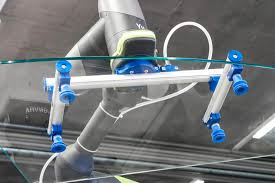
\includegraphics[scale=0.43]{./robotique_figures/vaccuum_gripper.png}
                \end{center}
                \begin{itemize}
                    \footnotesize
                    \item For \textbf{flat, smooth} surfaces
                    \item Multiple cups for large objects
                    \item \textbf{Venturi} or vacuum pump
                    \item Fast pick-and-place
                    \item Limited to non-porous materials
                \end{itemize}
            \end{block}
        \end{column}
        
        \begin{column}{0.48\textwidth}
            \begin{block}{Magnetic Grippers}
                \begin{center}
                    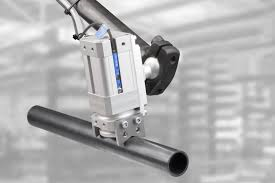
\includegraphics[scale=0.43]{./robotique_figures/magnetic_gripper.png}
                \end{center}
                \begin{itemize}
                    \footnotesize
                    \item For \textbf{ferrous metals}
                    \item Permanent or electromagnetic
                    \item No power needed for holding (permanent)
                    \item Can pick through paint/coating
                \end{itemize}
            \end{block}            
        \end{column}
    \end{columns}
    \textbf{Specialized Grippers}
                \begin{itemize}
                    \footnotesize
                    \item \textbf{Needle grippers:} For textiles
                    \item \textbf{Inflatable grippers:} For fragile items
                    \item \textbf{Electrostatic:} For wafers, glass
                    \item \textbf{Cryogenic:} For ice, frozen items
                \end{itemize}
\end{frame}

\begin{frame}{Tool End Effectors}
    \begin{columns}
        \begin{column}{0.48\textwidth}
        % --- SAME POSITION, OVERLAY SWITCHING ---
        \only<1>{
            \begin{block}{Welding Torches}
                \begin{center}
                    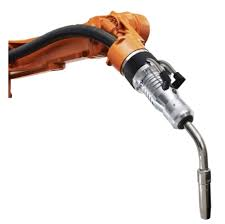
\includegraphics[scale=0.43]{./robotique_figures/welding_tool.png}
                \end{center}
                \begin{itemize}
                    \footnotesize
                    \item MIG, TIG, Spot welding
                    \item Wire feed, gas supply
                    \item Water cooling sometimes
                    \item Needs torch cleaning station
                \end{itemize}
            \end{block}
            }
            % --- SAME POSITION, OVERLAY SWITCHING ---
        \only<2>{
            \begin{block}{Dispensing Tools}
                \begin{center}
                    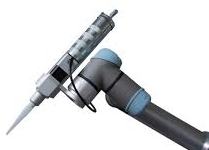
\includegraphics[scale=0.43]{./robotique_figures/dispensing_tool.png}
                \end{center}
                \begin{itemize}
                    \footnotesize
                    \item Glue, sealant, grease
                    \item Metering pumps
                    \item Need vision for path
                    \item Cleanup important
                \end{itemize}
            \end{block}
            }
        \end{column}
        
        \begin{column}{0.48\textwidth}
        % --- SAME POSITION, OVERLAY SWITCHING ---
        \only<1>{
            \begin{block}{Spindle Tools}
                \begin{center}
                    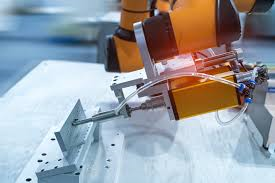
\includegraphics[scale=0.43]{./robotique_figures/spindle_tool.png}
                \end{center}
                \begin{itemize}
                    \footnotesize
                    \item Drilling, milling, routing
                    \item High-speed spindles
                    \item Automatic tool changers
                    \item Chip management
                \end{itemize}
            \end{block}
           }
           % --- SAME POSITION, OVERLAY SWITCHING ---
        \only<2>{ 
            \begin{block}{Other Common Tools}
                \begin{itemize}
                    \footnotesize
                    \item \textbf{Painting:} Spray guns, rotational atomizers
                    \item \textbf{Deburring:} Rotary files, brushes
                    \textbf{Measuring:} Probes, laser scanners
                    \textbf{Material Handling:} Forks, magnets, hooks
                    \textbf{Assembly:} Screwdrivers, nut runners
                \end{itemize}
            \end{block}
            }
        \end{column}
    \end{columns}
\end{frame}

\begin{frame}{End Effector Selection Considerations}

\begin{columns}[t]

    %--------------------- LEFT COLUMN ---------------------
    \begin{column}{0.48\textwidth}
        \begin{block}{Technical Factors}
            \footnotesize
            \begin{itemize}
                \item Part \textbf{geometry} and material
                \item Required \textbf{gripping force}
                \item \textbf{Cycle time} constraints
                \item Robot \textbf{payload} capacity
                \item Needed \textbf{accuracy} / repeatability
                \item \textbf{Environmental conditions:}
                \begin{itemize}
                    \footnotesize
                    \item Temperature
                    \item Cleanliness
                    \item Hazardous atmosphere
                \end{itemize}
            \end{itemize}
        \end{block}
    \end{column}

    %--------------------- RIGHT COLUMN ---------------------
    \begin{column}{0.48\textwidth}
        \begin{block}{Economic \& Practical Factors}
            \footnotesize
            \begin{itemize}
                \item End effector \textbf{cost}
                \item \textbf{Maintenance} needs
                \item \textbf{Changeover} time
                \item \textbf{Reliability} (MTBF)
                \item \textbf{Vendor support}
                \item \textbf{Integration} complexity
            \end{itemize}
        \end{block}
        \only<1>{
        \begin{alertblock}{Modern Trends}
            \scriptsize
            \begin{itemize}
                \item \textbf{Adaptive} (soft) grippers
                \item \textbf{Force sensing} fingertips
                \item \textbf{Vision-integrated} grasping
                \item \textbf{Quick-change} systems
                \item \textbf{Collaborative-safe} grippers
            \end{itemize}
        \end{alertblock}
        }
    \end{column}

\end{columns}

\vspace{2mm}
\only<2>{
\begin{exampleblock}{Rule of Thumb}
    \footnotesize
    End effector weight should be \textbf{$\leq 10\%$} of the robot’s rated payload.
\end{exampleblock}
}
\end{frame}



\begin{frame}{Summary: Complete Robot System}
    \begin{center}
      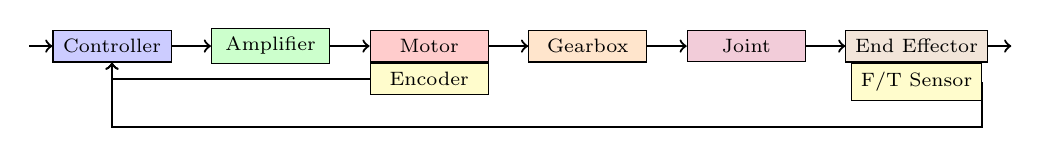
\begin{tikzpicture}[
    every node/.style={font=\scriptsize},
    node distance=0.5cm
]

% Main chain (narrow blocks)
\node[draw, rectangle, fill=blue!20, minimum width=1.5cm] (controller) {Controller};
\node[draw, rectangle, fill=green!20, right=0.5cm of controller, minimum width=1.5cm] (amplifier) {Amplifier};
\node[draw, rectangle, fill=red!20, right=0.5cm of amplifier, minimum width=1.5cm] (motor) {Motor};
\node[draw, rectangle, fill=orange!20, right=0.5cm of motor, minimum width=1.5cm] (gearbox) {Gearbox};
\node[draw, rectangle, fill=purple!20, right=0.5cm of gearbox, minimum width=1.5cm] (joint) {Joint};
\node[draw, rectangle, fill=brown!20, right=0.5cm of joint, minimum width=1.7cm] (ee) {End Effector};

% Sensors directly attached (no arrows between them)
\node[draw, rectangle, fill=yellow!20, below=0cm of motor, minimum width=1.5cm, anchor=north] (encoder) {Encoder};
\node[draw, rectangle, fill=yellow!20, below=0cm of ee, minimum width=1.5cm, anchor=north] (ftsensor) {F/T Sensor};

% Short arrows between main blocks
\draw[->, thick] (controller) -- (amplifier);
\draw[->, thick] (amplifier) -- (motor);
\draw[->, thick] (motor) -- (gearbox);
\draw[->, thick] (gearbox) -- (joint);
\draw[->, thick] (joint) -- (ee);

% Feedback paths (encoder + FT sensor to controller)
\draw[->, thick] 
    (encoder.west) -| ($(controller.south)+(0,-0.2)$) -- (controller);

\draw[->, thick]
    (ftsensor.east) |- ($(encoder.south)+(0,-0.4)$)
    -| (controller);

% External connections
\draw[<-, thick] (controller.west) -- ++(-0.3,0);
\draw[->, thick] (ee.east) -- ++(0.3,0);

\end{tikzpicture}


    \end{center}
    
    \vspace{5mm}
    \begin{columns}
        \begin{column}{0.5\textwidth}
            \begin{alertblock}{Key Takeaways}
                \begin{itemize}
                    \item Actuators provide motion
                    \item Sensors provide feedback
                    \item Transmissions match motor to load
                    \item End effectors do the work
                \end{itemize}
            \end{alertblock}
        \end{column}
        
        \begin{column}{0.5\textwidth}
            \begin{exampleblock}{System Integration}
                All components must work together seamlessly for optimal robot performance.
            \end{exampleblock}
        \end{column}
    \end{columns}
\end{frame}
\end{document}